\documentclass[a4paper, notitlepage]{article}
\usepackage{fullpage, listings, courier}
\usepackage[pdftex]{graphicx}
\usepackage{wrapfig}

\begin{document}

\title{IN4189 Software Reengineering \\ Assignment 2}
\author{Freek Post (1229540) \\ Borislav Todorov (4181840)}
\date{\today}
\maketitle

\section{Refactoring LwjglGL1Renderer}

In the previous assignment we discovered that the source code defining the rendering logic is quite complex and hard to understand. We think that the main problem that makes the source code so hard to understand is the violation of the SRP(Single Responsibility Principle). We discovered that all rendering logic resides in just a few classes which as a result encapsulate many different responsibilities. This has made the classes large in size, difficult to understand, maintain and extend. In this assignment we will improve the JME project by refactoring the logic for LWGLGL1 rendering. Currently, all this logic is encapsulated in the LwjglGL1Renderer class. 

First, before we started with the refactoring we used the \textbf{STAN} tool to measure some source code metrics which, at the end, are used to show that the refactoring has indeed improved the project. The measurements can be found bellow. One of the most important metrics is the Weighted Methods per Class(WMC). It has been introduced by Chidamber and Kemerer\footnote{Chidamber, S.R. and Kemerer, A Metrics Suite for Object Oriented Design, Software Engineering, IEEE Transactions on, 1994 } and indicates the complexity of classes. Classes with high WMC are potential candidates to be refactored into two or more classes.

\begin{itemize}
\item Classes : 1
\item Methods: 59
\item Attributes: 30
\item Lines of code: 940
\item WMC: 243
\end{itemize}

\subsection{Unit testing} 
The refactoring that we perform should improve the source code but it should not change the behaviour of the system. In order to make sure that it is not altered in any way we first devised a collection of unit tests for the affected class (LwjglGL1Renderer). This tests will prove that, at the end, we have preserved the behaviour of the system and we have not introduced any new problems.

The main challenge that we faced creating the tests was the fact that the class was tightly coupled to many other classes(Statistics, RendererContext, NativeObjectManager, Texture, Mesh, etc.) which made almost impossible to test the class. Therefore, the first thing that we did was to decouple the class from all the other classes. We did that by introducing interfaces of the dependent classes and referring to them instead of the concrete implementations. This enabled us to easily create mock objects and test the class on its own. 

Another interesting challenge was the fact that the class was coupled to the static methods of the GL11 class. In order to decouple the two classes we introduced a new interface(GL11Wrapper) and implementation(GL11WrapperImpl) that acts as an adaptor and wraps around the GL11 class. 

Next step was to create the actual unit tests. The challenge here was to decide what to validate in each test case. By further investigating the class we noticed that the class is a typical instance of the so called "manager" classes. It has almost no internal state and its main responsibility is to invoke methods of external classes(mainly GL11). Therefore, in the unit tests we validate the sequence and parameters of the called methods of these external classes. For example, executing the \textit{cleanup()} method results in the following sequence of method invocations: \textit{GL11.glColorMask(true, true, true); GL11.glDepthMask (true); GL11.glClear(17664)}.

When building the set of tests we aimed to reach maximum coverage. We used the \textbf{CodePro} tools in order to measure  the \textit{line} coverage of the test cases. At the end we managed to create 64 tests which cover 88.6\% of the class' source code.

All source code connected to the unit tests can be found under the \textit{jme3/test/com/jme3/renderer/lwjgl} folder.


\subsection{Refactoring}

As mentioned above, investigating the source code of the class we discovered that one of the main problems of the LwjglGL1Renderer is that it tries to combine many responsibilities into a single entity. As a result it has grown significantly in size and complexity. 

We started the refactoring by identifying different responsibilities at class level and extract the source code for each responsibility into a separate class. We ended up with the following responsibilities/classes which are also illustrated in Figure \ref{fig:1}:

\begin{itemize}
\item The logic for keeping track of the capabilities of the renderer was extracted to the \textbf{LwjglGL1Capabilities} class.
\item The logic for applying the light setting was extracted to the \textbf{LwjglGL1LightsRenderer} class.
\item The logic for rendering meshes was extracted to the \textbf{LwjglGL1MeshRenderer} class.
\item The logic for rendering textures was extracted to the \textbf{LwjglGL1TextureRenderer} class.
\item The logic for dealing with the view port was extracted to the \textbf{LwjglGL1ViewPort} class.
\item The logic for dealing with different projections was extracted to the \textbf{LwjglGL1Projection} class.
\item The logic for keeping track of and dealing with the glScissor was extracted to the \textbf{LwjglGL1Clipper} class.
\item The logic for for keeping track of the state of the renderer was extracted to the \textbf{LwjglGL1StateManager} class.
\end{itemize}

\begin{wrapfigure}{r}{0.5\textwidth}
\begin{center}
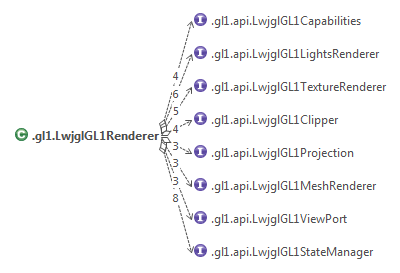
\includegraphics[width=0.50\textwidth]{graphics.png}
\end{center}
\caption{LWGLGL1 renderer decomposition. This diagram was reverse engineered with the \textbf{STAN} tool.}
\label{fig:1}
\end{wrapfigure} 


The end result is that all the logic is now distributed into 9 classes. The new role of the \textit{LwjglGL1Renderer} is just to act as a facade. It now contains almost no logic regarding the rendering process. In order to improve the system even more we continued by investigating the cohesion on method level. We noticed that there are several methods with significant size which suggests possible problems.

For example the LwjglGL1StateManager.\textbf{initialize} method is responsible to initialize the state of the renderer, load the capabilities, initialize the light settings, etc. This is a clear SRP violation and we divided the method into several methods for each responsibility. The case with the LwjglGL1LightsRenderer.\textbf{applyRenderState} and LwjglGL1LightsRenderer.\textbf{setLighting} methods was very similar and we refactored them using the same approach. 

All classes that compose the LwjglGL1 rendering logic can be found under the \textit{com.jme3.renderer.lwjgl.gl1} package.


\subsection{Evaluation}

In this assignment we refactored the JME in order to make it easier to understand, maintain and extend. This section focuses on improving the LwjglGL1Renderer by fixing the SRP violations. We believe that the refactoring is successful and significantly decreases the complexity of the source code. This statement is supported by the measurements bellow which were performed on the refactored source code. We managed to decrease the average methods per class by \textit{77\%}, attributes per class by \textit{84\%}, lines of code per class by \textit{88\%} and WMC per class by \textit{90\%}

\begin{itemize}
\item Classes : 11
\item Methods / class: 13.36
\item Attributes / class: 4.73
\item Lines of code/ class: 117
\item Average WMC: 24.5
\end{itemize}

\end{document}